\chapter{Theoretical Background}
\label{ch:theory}

This chapter is a \emph{visual-elements reference} for the rest of the thesis. Each section demonstrates one type of visual element supported by the document class, with a minimal but complete example that can be copied into another chapter. Where appropriate, the examples are drawn from the thesis topic --- attack-graph construction, blast-radius simulation, and defense optimization --- so that the chapter also serves as a worked example of the visual elements applied to a non-trivial domain.

\section{Attack Graphs and Their Visualization}

A figure is a floating environment that places a graphic at a suitable position on the page. The body of the figure is an \texttt{\textbackslash includegraphics} call (for a raster or vector image) or a TikZ picture. The image file must live in \texttt{img/} (or be referenced with a full path). The class \texttt{pclass.cls} also accepts an optional caption and label.

\begin{code}
	\begin{minted}{latex}
\begin{figure}[hbt!]
	\centering
	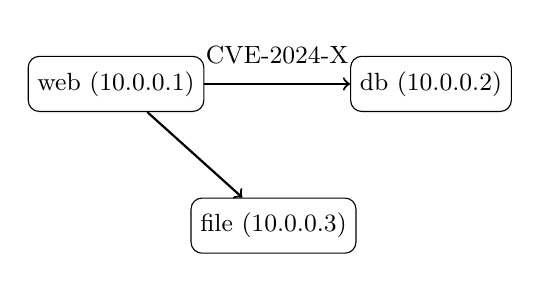
\begin{tikzpicture}[
		every node/.style={draw, rectangle, rounded corners, minimum width=2cm, minimum height=0.7cm, font=\small},
		arrow/.style={->, thick},
	]
	\node (h1) at (0, 1.2) {web (10.0.0.1)};
	\node (h2) at (4, 1.2) {db (10.0.0.2)};
	\node (h3) at (2, -0.6) {file (10.0.0.3)};
	\draw[arrow] (h1) -- node[above, draw=none, fill=none] {CVE-2024-X} (h2);
	\draw[arrow] (h1) -- (h3);
	\end{tikzpicture}
	\caption{Small attack graph: three hosts, two exploit edges.}
	\label{fig:attack-graph-example}
\end{figure}
	\end{minted}
	\caption{Source template for an attack-graph figure.}
	\label{src:theory:figure-template}
\end{code}

The example below uses the existing logo as a stand-in. In a real chapter, the image path would point at the actual result.

\begin{figure}[hbt!]
	\centering
	
\includegraphics[width=0.6\textwidth]{logo_wiisi.png}
	\caption{Placeholder figure: an attack-graph render produced by the system would replace this slot.}
	\label{fig:theory:figure-example}
\end{figure}

\section{Source Code Listings}

A source code listing is a floating environment based on \texttt{minted}. The class file \texttt{pclass.cls} defines a \texttt{code} environment that sets the listing type to \enquote{Source Code} and provides a caption and a label. The template (literal text, not active LaTeX) is:

\begin{quote}
	\texttt{\textbackslash begin\{code\}}\quad $\rightarrow$\quad \texttt{\textbackslash begin\{minted\}\{python\}}\quad $\rightarrow$\quad \emph{code body}\quad $\rightarrow$\quad \texttt{\textbackslash end\{minted\}}\quad $\rightarrow$\quad \texttt{\textbackslash caption\{...\}}\quad $\rightarrow$\quad \texttt{\textbackslash label\{src:...\}}\quad $\rightarrow$\quad \texttt{\textbackslash end\{code\}}
\end{quote}

\noindent A worked example in the Elixir language, showing a module that holds a single attack-graph node:

\begin{code}
	\begin{minted}{elixir}
defmodule NetworkDefense.AttackGraph.Node do
  @enforce_keys [:id, :host, :service, :vulnerabilities]
  defstruct id: nil, host: nil, service: nil, vulnerabilities: []

  def new(host, service, vulnerabilities) do
    %__MODULE__{
      id: "#{host}:#{service}",
      host: host,
      service: service,
      vulnerabilities: vulnerabilities
    }
  end

  def compromise_probability(%__MODULE__{vulnerabilities: vs}) do
    Enum.reduce(vs, 0.0, &max(&2, cvss_to_prob(&1.cvss)))
  end
end
	\end{minted}
	\caption{An attack-graph node module in Elixir.}
	\label{src:theory:elixir-example}
\end{code}

\noindent A worked example in the Python language, showing a min-cut finder on a tiny attack graph:

\begin{code}
	\begin{minted}{python}
def min_cut(graph, source, sink):
    """Stoer--Wagner min-cut, simplified for unweighted graphs."""
    remaining = set(graph.nodes)
    best_cut = float("inf")
    while len(remaining) > 1:
        weights = {n: 0 for n in remaining}
        in_tree = set()
        last, prev = None, None
        for _ in remaining:
            for n in remaining - in_tree:
                for (u, v) in graph.edges:
                    if u == n and v in in_tree:
                        weights[n] += 1
            chosen = max(remaining - in_tree, key=lambda n: weights[n])
            in_tree.add(chosen)
            prev, last = last, chosen
        cut = weights[last]
        if cut < best_cut:
            best_cut = cut
        graph = contract(graph, prev, last)
        remaining.remove(prev)
    return best_cut
	\end{minted}
	\caption{A min-cut implementation in Python.}
	\label{src:theory:python-example}
\end{code}

\section{Inline Code}

Inline code is typeset with \texttt{\textbackslash mintinline}. The first argument is the language, the second is the snippet:

\begin{itemize}
	\item \mintinline{elixir}|NetworkDefense.AttackGraph|
	\item \mintinline{elixir}|monte_carlo_step/3|
	\item \mintinline{python}|min_cut(graph, source, sink)|
\end{itemize}

\section{Tables}

The class loads \texttt{booktabs}, \texttt{multirow}, and \texttt{array}, so the standard patterns for academic tables are available. The simplest form is a three-column table with horizontal rules only:

\begin{table}[hbt!]
	\centering
	\begin{tabular}{lcr}
		\toprule
		\textbf{Strategy} & \textbf{Mean $|B|$} & \textbf{$p$-value} \\
		\midrule
		No defense     & 412 & ---      \\
		Random         & 388 & 0.21     \\
		CVSS-priority  & 274 & $< 0.01$ \\
		Proposed       & 153 & $< 0.01$ \\
		\bottomrule
	\end{tabular}
	\caption{Blast-radius comparison on a 200-host topology, $|V| = 200$.}
	\label{tab:theory:simple}
\end{table}

A wider table that combines \texttt{multirow} and \texttt{\textbackslash cline} is shown in Table~\ref{tab:theory:wide}. This is the pattern to use for benchmark results where a single row label spans multiple data rows.

\begin{table}[hbt!]
	\centering
	\begin{tabular}{lrrr}
		\toprule
		\textbf{Topology} & \textbf{Strategy} & \textbf{Mean $|B|$} & \textbf{Reduction ($\times$)} \\
		\midrule
		\multirow{2}{*}{Small (20 hosts)}  & No defense & 18  & 1.0  \\
		                                    & Proposed   & 5   & 3.6  \\
		\cline{2-4}
		\multirow{2}{*}{Large (1000 hosts)} & No defense & 980  & 1.0  \\
		                                    & Proposed   & 173  & 5.7  \\
		\bottomrule
	\end{tabular}
	\caption{Benchmark results on small and large topologies.}
	\label{tab:theory:wide}
\end{table}

\section{Diagrams with TikZ}

Diagrams are drawn with TikZ inside a \texttt{figure} environment. The example below is a small attack graph: each node is a host/service pair, and arrows show exploit opportunities. TikZ is sensitive to coordinate placement, so it is worth sketching the layout before committing to code.

\begin{figure}[hbt!]
	\centering
	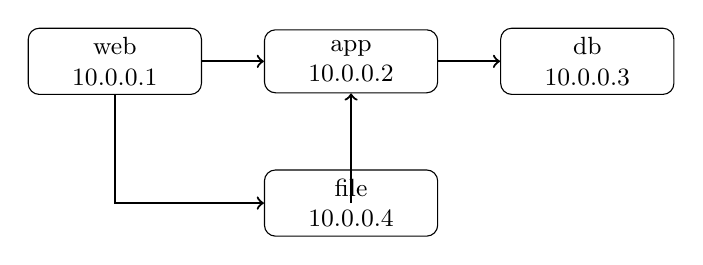
\begin{tikzpicture}[
			every node/.style={align=center, draw, rectangle, rounded corners, minimum width=2.2cm, minimum height=0.8cm, font=\small},
			arrow/.style={->, thick},
		]
		\node (a) at (0, 0)    {web\\10.0.0.1};
		\node (b) at (3.0, 0)  {app\\10.0.0.2};
		\node (c) at (6.0, 0)  {db\\10.0.0.3};
		\node (d) at (3.0, -1.8) {file\\10.0.0.4};

		\draw[arrow] (a) -- (b);
		\draw[arrow] (b) -- (c);
		\draw[arrow] (a) |- (d);
		\draw[arrow] (d) -| (b);
	\end{tikzpicture}
	\caption{Example TikZ diagram: a small attack graph.}
	\label{fig:theory:diagram}
\end{figure}

\section{Mathematics}

Inline math is delimited by \texttt{\$...\$} and display math by \texttt{\textbackslash[ ... \textbackslash]}. Equations can be numbered with the \texttt{equation} environment and aligned at a chosen relation with \texttt{align}.

Inline example: the probability that a single exploit of CVSS base score $s$ succeeds is $P = f(s)$, where $f$ is a monotone increasing function bounded above by $1$. The exact form of $f$ is an empirical question; one reasonable choice is $f(s) = s / 10$. Display example:

\[
P(\text{entry at } e \text{ reaches } v) \;=\; 1 - \prod_{(u, v) \in \text{path}} \bigl(1 - P(\text{exploit } (u, v))\bigr).
\]

Aligned example, useful for derivations:

\begin{align*}
	\mathrm{E}[B \mid e]  &= \sum_{h \in V} P(\text{reach } h \mid e) \\
	                      &= \sum_{h \in V} \Bigl( 1 - \prod_{(u, v) \in \pi_e(h)} \bigl(1 - f(s_{uv})\bigr) \Bigr).
\end{align*}

\section{Lists}

The class loads \texttt{enumitem}, which makes it easy to adjust list spacing. A simple itemized list:

\begin{itemize}
	\item Attack-graph construction.
	\item Monte Carlo blast-radius simulation.
	\begin{itemize}
		\item Stochastic propagation.
		\item Per-host compromise sampling.
	\end{itemize}
	\item Defense optimization.
\end{itemize}

A simple enumerated list:

\begin{enumerate}
	\item Ingest network topology.
	\item Enrich nodes with CVE / CVSS data.
	\item Build the attack graph.
	\item Run Monte Carlo simulation.
	\item Compute blast-radius map.
	\item Run optimizer (min-cut, greedy, or hybrid).
\end{enumerate}

A list with \texttt{\textbackslash enquote} strings around phrases:

\begin{itemize}
	\item The simulator is described as \enquote{stochastic, monotonic, and conservative}.
	\item The user provides \enquote{only the network topology and a CVE feed}.
\end{itemize}

\section{Quotes and Epigraphs}

A short quotation is set with the \texttt{quote} environment. The block is indented on both sides and the text is set in \enquote{quotation marks}:

\begin{quote}
	\itshape The best way to find out if a network is secure is to assume it isn't, and to ask what an attacker would do.
\end{quote}

The class also provides a local \texttt{\textbackslash epigraph} command that can be used inside a chapter to set an attributed quotation apart from the body text. The class file declares an \texttt{\textbackslash epigraph} macro from the \texttt{epigraph} package.

\begin{code}
	\begin{minted}{latex}
\epigraph{To be or not to be, that is the question.}{Shakespeare}
	\end{minted}
	\caption{Template for an in-chapter epigraph.}
	\label{src:theory:epigraph-template}
\end{code}

The rendered form is:

\epigraph{To be or not to be, that is the question.}{Shakespeare}

\section{Footnotes}

A simple footnote uses \texttt{\textbackslash footnote} and runs in the same paragraph as the reference. A footnote that is referenced from a position that is awkward for a marginal note (for example, after a list) can be deferred to the bottom of the page with \texttt{\textbackslash footnotetext} and a matching \texttt{\textbackslash footnote} placeholder.

A single-line footnote example: this is a sentence with a footnote\footnote{This is the footnote text; it appears at the bottom of the page.} attached.

A multi-line footnote using \texttt{\textbackslash footnotetext}:

\footnotetext{This is a longer footnote. It can span multiple lines, contain its own paragraph breaks, and even contain inline code such as \mintinline{elixir}|NetworkDefense.Optimizer.min_cut/2|, as long as the surrounding text is not overly fragile.}
